\section{Nube de Conductores}\label{section:NubeConductores}
El núcleo del sistema es una aplicación desplegada en la nube, la cual se ha
denominado \emph{Nube de Conductores}, donde se concentran en una base de datos
la información relativa a ciclistas y vehículos a motor. Un servicio de aplicación
web embebido llamado \emph{Jetty} se encarga de recibir y atender los mensajes
\Gls{http/1.1} que son enviados desde la parte de vehículos a motor y ciclistas.
Dos \emph{Handler} independientes se encargan de filtrar los mensajes que no han
sido correctamente construidos, es decir, tienen un formato inválido, e insertar
y actualizar los datos de la base de datos.

Para el despliegue de la aplicación se utilizado una máquina virtual \emph{Ubuntu Server
14.04 LTS} que cuenta con 2048 MiB de memoria RAM y 2 n\'ucleos para procesamiento.
También se ha reservado un dominio público para que las peticiones puedan ser enviadas
al servidor. Gracias a la herramienta \emph{ANT} se puede cambiar fácilmente la plataforma
donde se distribuya la aplicación, además esta configurada para poder ser ejecutada
directamente con el comando \emph{run}.

\begin{figure}[H]
	\begin{center}
		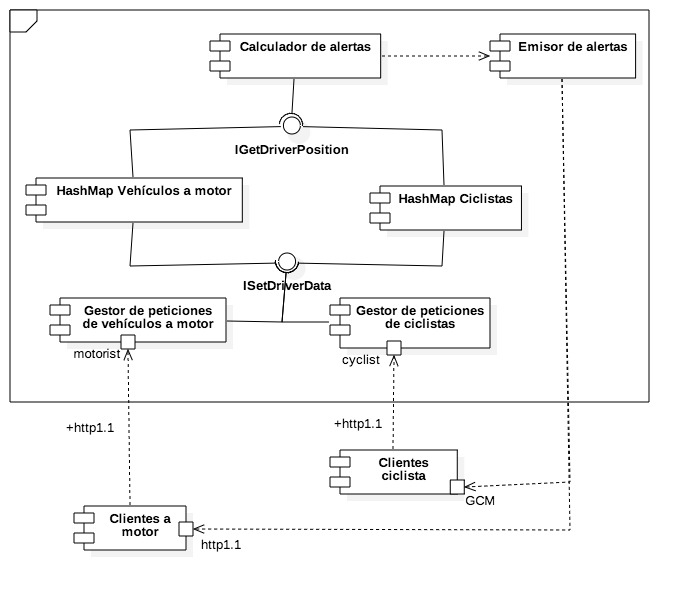
\includegraphics[scale=0.4]{DiagComponentes-Nube}
		\caption{Arquitectura de la Nube de Conductores}
		\label{fig:DiagComponentes-Nube}
	\end{center}
\end{figure}

\subsection{Procesos}\label{ssection:procesos}
A través del \gls{api} de \emph{Jetty} la aplicación crea un servidor con dos handler
de mensajes, uno para ciclistas y otro para vehículos a motor. A través de ellos la
\emph{Nube de Conductores} recibe datos de ciclistas y vehículos a motor, almacenándolos
en una base de datos interna sin necesidad de utilizar un DBMS, ya que no hace falta
que los datos sean persistentes más tiempo de lo que los vehículos estén emitiendo
su posición. Cada manejador posee un ThreadPool con el que crea un gestor para cada
mensaje recibido, este esta limitado a un número de hilos para evitar que la aplicación
se colapse.

Un registro se considera antiguo cuando no ha sido refrescado en un período de un
minuto. Para evitar que emplee información obsoleta, se ejecuta una rutina que tan
solo mantiene en memoria los registros que periódicamente están siendo actualizados;
ésto se realiza gracias al campo de \emph{timestamp}.

Paralelamente, cada vez que un mensaje es recibido en uno de los handler (conductores o
ciclistas), otro algoritmo compara la posición obtenida a través del handler con la de los
vehículos existentes. Si se detecta que algún ciclista ó vehículo a motor están próximos 
- en un rango menor a 200 metros - se manda a ambos vehículos una alerta avisándoles de 
su proximidad \emph{[Algoritmo \ref{alg:proximidadVehiculos}]}. En el apéndice
\ref{apendice:posicion_relative}, se detalla el funcionamiento del algoritmo que se encarga
de predecir si dos vehículos pueden encontrarse.

\begin{listing}
	\begin{minipage}{.4\textwidth}
		\begin{minted}[linenos=true]{java}
for (Motorist m : lMotorist) {
  for (Cyclist c : lCyclist) {
    if (isCollisionDanger(m, c)) {
      sendWarningToMotorist(c);
      sendCyclistPositionToMotorist(c);
    }
  }
}
		\end{minted}
	\end{minipage}
	\caption{Cálculo de la proximidad de los vehículos}\label{alg:proximidadVehiculos}
\end{listing}
